\chapter{Implementation}

    Following the specification, the aim of this chapter is to overview aspects of the implementation stage of the proposed \gls{alto} system.
    Firstly, attention is given in Section \ref{sec:implementation-technologies} to the chosen technologies that were leveraged to get the system from its specification stage into a working product.
    This includes tools and frameworks in the development and deployment phases, and whose choice greatly delimits the system's properties.
    Secondly, the server is put into spotlight in Section \ref{sec:implementation-server} by detailing how it is structured and how it behaves, taking special concern in how object oriented programming was leveraged to maximize modularity and reasoning of the system to facilitate future alterations and extensions.
    Brief implementation overviews are given to the Network Information Aggregator and Network State Providers in Section \ref{sec:implementation-aggregator} and Section \ref{sec:implementation-provider}, respectively, commenting where they are similar and where they differ from the \gls{alto} server's implementation.

\section{Technologies used}

\label{sec:implementation-technologies}

    Starting the implementation stage of every project, attention must be given into what tools are selected to make it come to fruition.
    These can greatly impact the success of the developed software, and has concrete consequence in its maintenance and future extension.

    The specified system architecture is composed by key entities whose interactions among themselves are clearly defined by interfaces.
    More so, considering the example deployment scenarios, its evident that each entity resides in different topological regions throughout the network, with the \gls{alto} server, clients, and status providers being scattered throughout an \gls{isp} domain.
    Each entity can then be thought of as a self-contained system in of itself who must abide by the proposed interfaces to properly work on the system.
    A logical conclusion to this is that each entity implementation is independent from the next, needing to only assure a common communication channel that all entities within it can properly understand.
    This gives great flexibility in the system implementation as a whole, because different tools can be leveraged to different entities if needed, and such entities that be worked on independently from the rest without impacting the function of the group.

    Regarding the \gls{alto} server, first attention is given to the \gls{alto} resources that must be provided by it.
    They all share some common properties, such as resource id, \glspl{acl}, owner, etc., and functionality, such as the ability to be read and updated, or their permissions modified.
    This similarity is further intensified within groups of resource types, more specifically cost maps. 
    In these resources, the only concrete difference between and endpoint and a \gls{pid} cost map is the type of entity the costs refer to, which are endpoint and \gls{pid} addresses, respectively.
    The sequence of steps that must be taken from the initial point where a client requests a resource up until that resource is provided can be abstracted as the sequential interaction between concrete modules that have a given, self contained, purpose, and communicate with a common interface.
    This is an architectural pattern that is a micro version of the one existing in the system, that shares all its properties that were discussed previously.
    Some of these modules would include client request monitoring, its parsing, its validation, database retrieval, database storage, and serialization.
    With all this in mind, an object-oriented programming seems like a proper fit for the complexity pertaining to the \gls{alto} server, especially considering how future extensions would be likely, as very much will be in case of the \gls{alto} working group.
    By working with objects as the base programming entity, many of the highlighted similarities between resources will become easy to be put into evidence, and module encapsulation and interfacing are natural and thus arguably easier to develop and maintain.
    Importance is also placed in choosing a compiled language that is statically typed.
    This is due to the fact that a compiled language favors performance over an interpreted alternative, which seems favourable for the expected scale of the \gls{alto} system, and typed constrictions provide needed structure verifications that aid in the programmer's confidence in its reliability, and often helps reduces mistakes.
    The language choice finalizes with Java \cite{java}, which matches the given requirements and is the one with most prior personal development experience, coupled with its maturity and wide access to libraries and frameworks.

    The Java Spring framework \cite{java-spring} is a main component of the developed server software. 
    The framework's inversion of control paradigm allows dependencies to be managed through configuration files and annotations to identify objects to be scanned by the framework, providing a means of development that is quite flexible, reduces boilerplate code, and favors loose coupling between objects, facilitating the independent development of implementations that can themselves be changed in the future with little consequence to the entire system, given that they implement the stipulated interface.
    Adding to this, the Spring framework provides modules that are very much needed for the server implementation, namely for \gls{mvc} architectures, \gls{http}-based \gls{rest} \glspl{api}, authentication and authorization, data access, and both unit and integration testing, to name a few.
    Given that other frameworks could provide similar functionality, Spring was favored due to its development team's focus on performance and flexibility, and because the framework has continuous development support and an increased community popularity, all of this raising the odds that this framework becomes maintained throughout the future, in comparison to some that have since lost support.

    Finally, focus was given for database-related decisions.
    Since resource manipulation through the \gls{rest} \glspl{api} revolve around \gls{json} manipulation, a preference was made for a database that allows the resources to be saved in a similar fashion, thereby reducing a layer of abstraction that makes reasoning on the software easier.
    Considering the scale at which an \gls{alto} server might be subjected to requests, a database that favors performance seems like a better choice, in particular one that easily allows for horizontal scaling.
    A last consideration is made for a database that is schema-less, since for the network information aggregation server, a myriad of types of data can be added by state providers to account for the huge variety of protocols and standards that retrieve network information, and more can exist in the future that weren't initially pondered by the \gls{isp} administrator, as more network protocols and data properties become relevant to attain, so a flexibility in what can be stored seems more appropriate.
    In a similar vein, for the \gls{alto} server, the \gls{alto} protocol itself has been subject to continuous changed that still aim for legacy support, it can be argued that future changes will be common, and doing so without increased server downtime - something that would be required by schema-driven databases - seems favorable considering the scale and importance of an \gls{alto} service.
    The existence of private properties whose scope is outside of the protocol and can be freely defined by the user, while not impossible to implement with a schema, seems to lend itself more naturally to a schema-less design.
    With all these considerations in mind, a database that abides to these constrictions and has a healthy developer support and user adoption is MongoDB \cite{mongodb}, which was chosen.

    As per security, the same philosophy of the \gls{alto} working group will be used and pre-existing, mature technologies will be leveraged.
    \gls{https} will be used over base \gls{http} as a communication protocol between entities as a means to resolve many of the identified threats.
    By using certificates with \gls{https}, the server entity authentication can be assured, and through the usage of \gls{tls} as a cryptographic security tool, both confidentiality and integrity are secured via data encryption and digest calculation, respectively.
    As per client authentication, a deliberate choice was made to use \gls{http} basic \cite{http-basic}, as opposed to \gls{http} digest \cite{http-digest} that is demanded by the base \gls{alto} working group's specification.
    With basic authentication, user and password fields are sent in encoded - not encrypted - fashion, and such information is firstly validated by the server that, if the attempt is successful, proceeds with its normal operation.
    Due to the lack of encryption, this method of client authentication will be complemented with the usage of \gls{https} to provide a secure communication channel that would otherwise be open to credential exposure and tampering.
    The working group's suggested digest method hashes the credentials by using a nonce - a number to be used only once - that was provided by the server, thus also protecting against data exposure and tampering.
    However, since \gls{https} will be leveraged, there's no need to have an authentication system that does much more beyond of what \gls{http} basic does, therefore facilitating client applications and giving the server flexibility on how they wish to store user credentials, since the basic authentication allows one to store the hash of passwords alone, whereas digest requires the storage of the hash value of "username:password:realm".
    These and other comparisons between these authentication methods are available at \cite{http-authentication} and further helped in the decision.


\section{Server architecture}

    \label{sec:implementation-server}

    The macro-level architectural diagram specified that the server's role is to serve incoming requests by clients and providers, and to interface with a database to persist resource storage.
    The server will implement a \gls{rest} interface leveraging the \gls{http} as this pair is widely accepted and ubiquitous on the Internet, but also due to the fact that its resource-oriented interface standards fit nicely into the specified interface for \gls{alto} server interactions, which too revolve around resource manipulation, and by adhering to proper \gls{rest} designs good scalability can be achieved due to its stateless nature and potential for resource caching.
    The choice of \gls{http} as an application protocol fits nicely into a philosophy of leveraging existing and well proven protocols and technologies to increase the project's success, and indeed so was done to integrate authentication and encryption mechanisms.

    To accomplish this interface implementation, the internal server architecture will utilize the \gls{mvc} design pattern.
    This three-layered architecture consists firstly by a controller layer that intercepts communication requests, which after parsed and validated are redirected to the business layer, which in turn employs business logic to help satisfy the controller's requests, which may require a subsequent layer descent into the data layer via database queries.

    Figure \ref{fig:controller-unversioned-architecture} displays a class diagram focusing on controller classes that deal with resources that are not susceptible to version control - this includes every resource except the network map.
    As can be seen, all concrete controllers - such as an endpoint property map controller - are extensions to a generic controller class that is parametrized by its \gls{dto} , filter \gls{dto}, and service instances.
    This design choice was made because all controller logic that regards to resources without version control are the same, and by creating generic classes with type parametrization code reutilization is increased.
    The parametrization required by the controller is required to pass a concrete instance of the unversioned resource service generic class, which in of itself requires parametrization in resource \gls{dto} and resource filter \gls{dto}.
    By reflecting on common controller and service behaviour between all version control lacking resources, the conclusion was that working around generic classes maximizes reutilization, facilitates reasoning and decreases potential error.

\begin{figure}[h]
\centering
\hspace*{-3em}
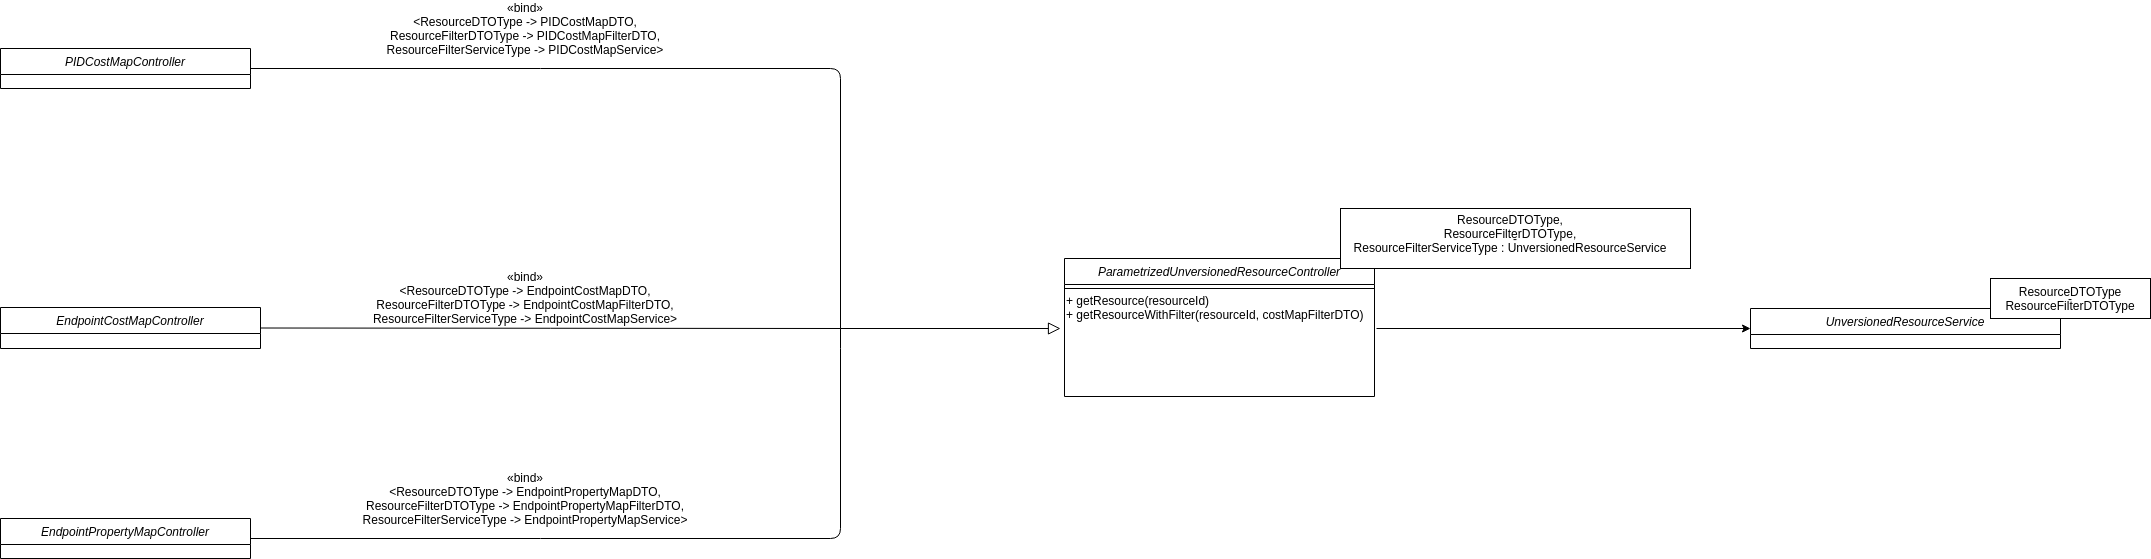
\includegraphics[scale=0.23]{img/controller-unversioned-architecture.png}
\caption{Controller layer class architecture}
\label{fig:controller-unversioned-architecture}
\end{figure}

    To help better visualize the result, refer to how the generic controller is implemented in Listing \ref{lst:generic-unversioned-controller}.
    To retrieve a resource, simply call the service class with or without the proper filter, depending on which method was triggered, by calling the appropriate methods that must implement the resource service interface.
    For example, an endpoint property map controller implementation simply extends the generic controller by providing the concrete \gls{dto}, filter \gls{dto}, and service implementations, as seen in Listing \ref{lst:endpoint-property-map-controller}.

\begin{center}
\begin{tabular}{H}
\begin{lstlisting}[frame=tlrb, caption=Parametrized Controller class for unversioned resources, label={lst:generic-unversioned-controller}, basicstyle=\tiny]
public class ParametrizedUnversionedResourceController
    <ResourceDTOType,
     ResourceFilterDTOType,
     ResourceServiceType extends ALTOUnversionedResourceService
                                        <ResourceDTOType,
                                         ResourceFilterDTOType>
     > {

    private final ResourceServiceType resourceService;

    @Autowired
    public ParametrizedUnversionedResourceController(ResourceServiceType resourceService) {
        this.resourceService = resourceService;
    }

    @PreAuthorize("@ResourceAuthorizationService.hasPermission(authentication, #resourceId, T(com.example.restservice.dto.security.PermissionDTO).READ)")
    @RequestMapping(method = RequestMethod.GET, value = "{id}")
    public ResourceDTOType getResource(@PathVariable(value = "id") String resourceId) {
        return resourceService.getResource(resourceId);
    }

    @PreAuthorize("@ResourceAuthorizationService.hasPermission(authentication, #resourceId, T(com.example.restservice.dto.security.PermissionDTO).READ)")
    @RequestMapping(method = RequestMethod.POST, value = "{id}")
    public ResourceDTOType getCostMapWithFilter(@PathVariable(value = "id") String resourceId,
                                                @Valid @RequestBody ResourceFilterDTOType costMapFilterDTO) {
        return resourceService.getResource(resourceId, costMapFilterDTO);
    }
}

\end{lstlisting}
\end{tabular}
\end{center}

\begin{center}
\begin{tabular}{H}
\begin{lstlisting}[frame=tlrb, caption=Concrete controller extending from a parametrized one, label={lst:endpoint-property-map-controller}, basicstyle=\tiny]
@RestController
@RequestMapping("endpointprops")
public class EndpointPropertyMapController
    extends ParametrizedUnversionedResourceController<EndpointPropertyMapDTO, EndpointPropertyMapFilterDTO, EndpointPropertyMapService> {

    @Autowired
    public EndpointPropertyMapController(EndpointPropertyMapService resourceService) {
        super(resourceService);
    }
}
\end{lstlisting}
\end{tabular}
\end{center}

    The same reasoning was used to implement the network map controller, but since this is the only resource that accepts versioning, the correspondent generic controller behavior does not contain similar behavior to the one above, and thus another was created, as seen in Listing \ref{lst:generic-versioned-controller}.
    The service layer implementation must now let the controller retrieve either a specific version of a resource, or the most recent one if no version is specified by the client.


\begin{center}
\begin{tabular}{c}
\begin{lstlisting}[frame=tlrb, caption=Parametrized controller class for versioned resources, label={lst:generic-versioned-controller}, basicstyle=\tiny]
public class ParametrizedVersionedResourceController
    <ResourceDTOType,
     ResourceFilterDTOType,
     ResourceServiceType extends ALTOVersionedResourceService
                                        <ResourceDTOType,
                                         ResourceFilterDTOType>
> {

private final ResourceServiceType resourceService;

@Autowired
public ParametrizedVersionedResourceController(ResourceServiceType resourceService) {
    this.resourceService = resourceService;
}

@RequestMapping(method = RequestMethod.GET, value = "{id}")
@PreAuthorize("@ResourceAuthorizationService.hasPermission(authentication, #resourceId, T(com.example.restservice.dto.security.PermissionDTO).READ)")
public ResourceDTOType getVersionedResource(@PathVariable(value = "id") String resourceId,
                                            @RequestParam(value = "version", required = false) String resourceVersion) {
    return resourceVersion != null
            ? resourceService.getResourceVersion(resourceId, resourceVersion)
            : resourceService.getLatestResourceVersion(resourceId);
}

@PreAuthorize("@ResourceAuthorizationService.hasPermission(authentication, #resourceId, T(com.example.restservice.dto.security.PermissionDTO).READ)")
@RequestMapping(method = RequestMethod.POST, value = "{id}")
public ResourceDTOType getVersionedResourceWithFilter(@PathVariable(value = "id") String resourceId,
                                                      @RequestParam(value="version", required = false) String resourceVersion,
                                                      @Valid @RequestBody ResourceFilterDTOType resourceFilter) {
    return resourceVersion != null
            ? resourceService.getResourceVersion(resourceId, resourceVersion, resourceFilter)
            : resourceService.getLatestResourceVersion(resourceId, resourceFilter);
    }
}
\end{lstlisting}
\end{tabular}
\end{center}

    The purpose of some pieces of the shown code isn't immediately obvious, and will be now further explained.
    Starting with input validation, the usage of the "@Valid" annotation on an endpoint controller parameter signifies that the framework must initialize a validator class that should examine and validate that input against the defined rules.
    The rules are defined on the \gls{dto} class that is to be passed by the client into the server, and validation annotations from the framework are leveraged to define attribute-specific rules.
    Listing \ref{lst:cost-map-dto}, for example, includes the "@JsonProperty" annotation that defines optional and obligatory fields in the de-serialization step, and whenever needed more types of attribute validation annotations were used, including non-blank strings, non negative integers, and values within a certain non continuous set of possibilities.

\begin{center}
\begin{tabular}{c}
\begin{lstlisting}[frame=tlrb, caption=Cost map DTO class, label={lst:cost-map-dto}, basicstyle=\tiny]
@Document(collection = "CostMaps")
public class CostMapDTO {

    @JsonIgnore
    @Id
    private String id;

    @NotNull
    @Indexed(unique = true)
    @Field("meta")
    private MetaDataDTO metaDataDTO;

    @NotNull
    @Field("cost-map")
    private Map<String, Map<String, Integer>> costMappings;

    @JsonCreator
    public CostMapDTO(@JsonProperty(value = "meta", required = true) MetaDataDTO metaDataDTO,
                      @JsonProperty(value = "cost-map", required = true) Map<String, Map<String, Integer>> costMappings) {
        this.metaDataDTO = metaDataDTO;
        this.costMappings = costMappings;
    }

    public String getId() {
        return id;
    }

    public void setId(String id) {
        this.id = id;
    }

    public MetaDataDTO getMetaDataDTO() {
        return metaDataDTO;
    }

    public void setMetaDataDTO(MetaDataDTO metaDataDTO) {
        this.metaDataDTO = metaDataDTO;
    }

    public Map<String, Map<String, Integer>> getCostMappings() {
        return costMappings;
    }

    public void setCostMappings(Map<String, Map<String, Integer>> costMappings) {
        this.costMappings = costMappings;
    }
}
\end{lstlisting}
\end{tabular}
\end{center}


    For class-wide validation, custom validator classes were created and afterwards annotated into the class in question.
    For example, for the cost map filter \gls{dto}, which defines the filter that is passed by the client whenever cost map filtering is selected, a custom validator class was created and annotated with "@ValidCostParametrization".
    This class implements the class-wide restrictions imposed in the \gls{alto} protocol regarding cost map filters, which dictate that a user can only select either a single or multi-cost map request, and whenever calendarization is requested, the total count of cost types requested must match the number of flags that dictate if a given cost type must provide its calendar form.
    Assuring both attribute and class-wide rule definition and enforcement, the system can validate all user input to maintain system correctness.

    Another element from the shown controller implementation is the "@PreAuthorize" annotation.
    These, and similar others, are part of the Spring security module and serve as constriction setters that, if not successful, do not let the annotated method be executed.
    This is the basis for access control in the server system, as is shown in Listing \ref{lst:generic-versioned-controller}, retrieving a resource using the GET method requires that a given constraint is verified.
    This constraint verification process is handled by a specially created authorization service that receives authentication information, the resource id in question, and what action is being requested - in this case being "READ".
    This is how all access control restrictions upon \gls{alto} resources is implemented - with uploaded resources containing an \gls{acl} mapping user roles to allowed actions, all controller access must first verify that the given authorized user is authorized to perform that action.
    The authorization service, seen on Listing \ref{lst:authorization-service}, exposes a "hasPermission" method in its interface and is tasked with confirming if the following action is allowed considering the system's constrictions and the upload entity's defined access control rules.

\begin{center}
\begin{tabular}{c}
\begin{lstlisting}[frame=tlrb, caption=Excerpt of the resource authorization service, label={lst:authorization-service}, basicstyle=\tiny]
@Service("ResourceAuthorizationService")
public class SingleProviderResourcePermissionsResourcesAuthorizationService implements ResourcesAuthorizationService {

        public boolean hasPermission(Authentication authentication, String resourceId, PermissionDTO permissionDTO) {

        if (authentication instanceof AnonymousAuthenticationToken) {
            // User must be authenticated
            return false;
        } else {
            // Get roles the user has attributed to him
            List<String> userRoles = getRoleNames(authentication.getAuthorities());

            return hasGeneralActionPermission(userRoles, permissionDTO)
                && hasResourcePermissions(userRoles, resourceId, permissionDTO);
        }
    }


/*
* Implementation
*/
}
\end{lstlisting}
\end{tabular}
\end{center}


    Simply put, for a service to validate a request it must validate that the following are all true: a) the user is authenticated; b) the user has general system access to the system with that action and c) the user has concrete access to that resource with that action.
    By creating an additional access layer to the system that is separate from the resource's access list, the server can apply both a per-role and per-resource access control, allowing more control for server administrators outside of what the resource \gls{acls} dictate.
    Because of this, it's possible, for example, to completely blacklist a given role from a system even if a resource upload entity allows him with his \gls{acl}.

    As per the service layer, a similar philosophy to the controller was taken - i.e., to expose behavior similarities and utilize generic types to inject dependency implementations, and an equal class structure exists.  
    Much like the controller architecture, by isolating common patterns one can minimize code repetition and promote function modularity, and this results in faster development in less errors that could result in redundant logic being applied.
    Service classes leverage resource repositories and mapper classes that translate an entity into a transfer object, which is a helpful design decision that decouples class implementation from representation, allowing the system to comply to the defined protocol without the restriction of storing and handling it the same way within the system.
    A versioned service is quite similar, but exposes an interface that lets the caller retrieve resources considering their version tag, or simply retrieve the most recent version.

    As an example, Listing \ref{lst:cost-map-service} shows the cost map service implementation, that simply extends the parametrized class and injects the implementations specific to how a cost map service must behave - i.e., how it stores and how it translates resources.
    It then adds only methods specific to their service implementation that aren't shared among others - in this case, how to retrieve a resource with a given cost map filter, which requires different actions depending on whether or not the filter specifies a single or multi cost request.

\begin{center}
\begin{tabular}{c}
\begin{lstlisting}[frame=tlrb, caption=Cost map service class, label={lst:cost-map-service}, basicstyle=\tiny]
@Component
public class CostMapServiceImpl extends ALTOGenericResourceRepoService<CostMapEntity,
                                                                       CostMapProjection,
                                                                       CostMapDTO,
                                                                       CostMapRepository,
                                                                       CostMapMapper>
                                implements CostMapService {

    private CostMapFilterMapper costMapFilterMapper;

    @Autowired
    public CostMapServiceImpl(CostMapRepository costMapRepository,
                              CostMapMapper costMapMapper,
                              CostMapFilterMapper costMapFilterMapper) {
        super(costMapRepository, costMapMapper);
        this.costMapFilterMapper = costMapFilterMapper;
    }

    @Override
    public Optional<CostMapDTO> getResourceWithFilter(String resourceId, String resourceVersion, CostMapFilterDTO costMapFilterDTO) {
        CostMapProjection costMapProjection = costMapFilterMapper.mapFrom(costMapFilterDTO);
        Optional<CostMapEntity> optionalCostMapEntity = resourceRepository.findVersionOfResourceWithProjection(resourceId, resourceVersion, costMapProjection);
        return optionalCostMapEntity.map(costMapEntity -> resourceMapper.mapVersionAtPosition(costMapEntity, 0));
    }

    @Override
    public Optional<CostMapDTO> getLatestResourceWithFilter(String resourceId, CostMapFilterDTO costMapFilterDTO) {
        CostMapProjection costMapProjection = costMapFilterMapper.mapFrom(costMapFilterDTO);
        Optional<CostMapEntity> optionalCostMapEntity = resourceRepository.findLatestVersionOfResourceWithProjection(resourceId, costMapProjection);
        return optionalCostMapEntity.map(costMapEntity -> resourceMapper.mapVersionAtPosition(costMapEntity, 0));
    }
}
\end{lstlisting}
\end{tabular}
\end{center}


    The mapper classes, mentioned above, are tasked with mapping between two different representations of a class.
    Specifically, mapper classes are used in the server to map between protocol representations of a resource or a filter, into representations to be used internally.
    Like previously mentioned, decoupling protocol and internal class representations makes the resources easier to store, as they can be translated into a form more ideal for MongoDB storage - in some cases making some queries quite impossible to achieve otherwise - and easier to handle, since protocol representation of data is better for data transmission and user readability, but not as much for querying and algorithmically processing.
    For example, the protocol representation of calendarized cost maps separates the cost information, cost values and calendar information into three separate lists, and their matching must be made by equal index access.
    Working internally with a data structure that is optimized for simpler and quicker data handling and querying can optimize application performance and reduce code complexity, being a good compromise for the added mapping layer that is consequentially required.
    As an example, Listing \ref{lst:costmap-comparison} display how a calendar cost map is represented in the \gls{alto} protocol versus that same content as a storage-ready entity.
    Whilst still storing the same information, changing how it's laid out cold facilitate human reading and client parsing for a display-oriented usage in the protocol representation, and facilitate traversal and general database query for a storage-oriented usage.


\begin{center}
\begin{minipage}[t]{.43\textwidth}
\begin{lstlisting}[frame=lrbt, basicstyle=\tiny]
  /calendar/costmap/filtered
  HTTP/1.1 200 OK
  Content-Length: 1043
  Content-Type: application/alto-costmap+json

  {
    "cost-type" : {
      "cost-mode" : "numerical",
      "cost-metric" : "routingcost",
    },
    "calendar-responde-attributes" : [
      {
        "calendar-start-time" : "Tue, 1 Jul 2019 13:00:00 GMT",
        "time-interval-size" : 7200,
        "number-of-intervals" : 12
      },
    ],
    "cost-map" : {
      "PID1" : {
        "PID1" : [ 1, 12, 14, 18, 14, 14, 14, 18, 19, 20, 11, 12],
        "PID2" : [ 13, 4, 15, 16, 17, 18, 19, 20, 11, 12, 13, 14],
        "PID3" : [ 20, 20, 18, 14, 12, 12, 14, 14, 12, 12, 14, 16]
      }
    }
  }
\end{lstlisting}
\end{minipage}\hfill
\begin{minipage}[t]{.54\textwidth}
\begin{lstlisting}[frame=lrbt, basicstyle=\tiny]
{
  "resourceId" : "filtered",
    "mappingEntities": [
    {
      "costMode": "numerical",
      "costMetric": "routingcost",
      "calendarAttributesEntity": {
        "startTime": "Tue, 1 Jul 2019 13:00:00 GMT",
        "intervalSize": 7200,
        "intervalNumber": 12,
        "iterations": 1
      },
      "fromSrcCostEntities": [
      {
        "srcNode": "PID1",
        "dstCostEntities": [
        {
          "dstNode": "PID1",
          "calendaredCostValues": [1, 12, 14, 18, 14, 14, 14, 18, 19, 20, 11, 12]
        },
        {
          "dstNode": "PID2",
          "calendaredCostValues": [13, 4, 15, 16, 17, 18, 19, 20, 11, 12, 13, 14]
        },
        {
          "dstNode": "PID3",
          "calendaredCostValues": [20, 20, 18, 14, 12, 12, 14, 14, 12, 12, 14, 16]
        }
        ]
        }
      ]
      }
  ]
}
\end{lstlisting}
\end{minipage}
\captionof{lstlisting}{Example calendar cost map in protocol and database representation}
\label{lst:costmap-comparison}
\end{center}

    Data access is materialized in the form of repository classes, responsible for providing an interface for service classes that let them retrieve entity classes from the database, doing so by generating the required queries to the Mongo database.
    Again, for behaviour similarity exposure, the repositories inherit from a base versioned and unversioned repository that compiles the queries needed to retrieve resources, requiring the inheriting repositories to specify additional implementation-specific queries needed to extend upon the functionality.
    For this to be possible, entity representation on the database must too be similar, so the base queries, when applied to either a network map or an endpoint property map, which are two unversioned example resources, can work the same.
    Listing \ref{lst:costmap-vs-endpoint-prop} shows an example database representation of a cost map and an endpoint, respectively.
    Notice how common properties are indexed in the same way, and only differ on implementation-specific details.
    The "resourceId" attribute can be queried and the "mappingEntities" attribute can be loaded by the high-level query without needing to know what concrete resource entity is being treated, and further implementation-specific querying is made by the inheriting repositories.

\begin{center}
\begin{minipage}[t]{.43\textwidth}
\begin{lstlisting}[frame=lrbt, basicstyle=\tiny]
{
  "resourceId" : "my-default-cost-map",
  "mappingEntities": [
    {
      "addressType" : "IPV4",
      "addressValue" : "192.0.2.34",
      "endpointPropertyEntities" : [
        {
          "propertyType" : "my-default-network-map.pid",
          "propertyValue" : "PID1"
        },
        {
          "propertyType" : "geolocation",
          "propertyValue" : "123132;33231"
        }
      ]
    }
  ]
}
\end{lstlisting}
\end{minipage}\hfill
\begin{minipage}[t]{.54\textwidth}
\begin{lstlisting}[frame=lrbt, basicstyle=\tiny]
{
  "resourceId" : "filtered",
    "mappingEntities": [
    {
      "costMode": "numerical",
      "costMetric": "routingcost",
      "calendarAttributesEntity": {
        "startTime": "Tue, 1 Jul 2019 13:00:00 GMT",
        "intervalSize": 7200,
        "intervalNumber": 12,
        "iterations": 1
      },
      "fromSrcCostEntities": [
      {
        "srcNode": "PID1",
        "dstCostEntities": [
        {
          "dstNode": "PID1",
          "calendaredCostValues": [1, 12, 14, 18, 14, 14, 14, 18, 19, 20, 11, 12]
        },
        {
          "dstNode": "PID2",
          "calendaredCostValues": [13, 4, 15, 16, 17, 18, 19, 20, 11, 12, 13, 14]
        },
        {
          "dstNode": "PID3",
          "calendaredCostValues": [20, 20, 18, 14, 12, 12, 14, 14, 12, 12, 14, 16]
        }
        ]
        }
      ]
      }
  ]
}
\end{lstlisting}
\end{minipage}
\captionof{lstlisting}{Similar structure in a costmap and endpoint property map storage entities}
\label{lst:costmap-vs-endpoint-prop}
\end{center}

    Listing \ref{lst:network-map-repository} shows a portion of the network map repository implementation.
    To retrieve a specific version of a resource, build query methods are retrieved from the versioned repository class, and network map specific processing is added to apply network map projections, which in this case means retrieving only the specified \glspl{pid}.


\begin{center}
\hspace*{-0.4em}
\begin{tabular}{c}
\begin{lstlisting}[frame=tlrb, caption=Network map repository, label={lst:network-map-repository}, basicstyle=\tiny]
@Repository
public class NetworkMapMongoRepository extends VersionedResourceMongoRepository<NetworkMapEntity>
                                            implements NetworkMapRepository {

    public NetworkMapMongoRepository(MongoTemplate mongoTemplate) {
        super(NetworkMapEntity.class, mongoTemplate);
    }

    private Optional<List<AggregationOperation>> givenSingleVersionOfResourceBuildProjectionAggregationOperations(NetworkMapProjection networkMapProjection) {
        if (networkMapProjection.getSrcPIDs().isPresent()) {
            return Optional.of(
                    Arrays.asList(
                            unwind("mappingEntity.addressAggregationEntities"),
                            match(Criteria.where("mappingEntity.addressAggregationEntities.pid").in(networkMapProjection.getSrcPIDs().get())),
                            group()
                                    .first("resourceId").as("resourceId")
                                    .first("mappingEntity.versionTag").as("versionTag")
                                    .push("mappingEntity.addressAggregationEntities").as("addressAggregationEntities"),
                            project("resourceId")
                                    .and("versionTag").as("mappingEntity.versionTag")
                                    .and("addressAggregationEntities").as("mappingEntity.addressAggregationEntities")
                    )
            );
        } else {
            return Optional.empty();
        }
    }

    private List<AggregationOperation> buildFindResourceAggregationOperations(String resourceId, String versionTag, NetworkMapProjection projection) {
        List<AggregationOperation> aggregationOperations = new ArrayList<>();

        if (versionTag != null) {
            aggregationOperations.addAll(buildGetVersionOfResourceAggregationOperations(resourceId, versionTag));
        } else {
            aggregationOperations.addAll(buildGetLatestVersionOfResourceAggregationOperations(resourceId));
        }

        givenSingleVersionOfResourceBuildProjectionAggregationOperations(projection).ifPresent(aggregationOperations::addAll);

        aggregationOperations.add(getWrapVersionInsideArrayOperation());

        return aggregationOperations;
    }

    private List<AggregationOperation> buildFindResourceAggregationOperations(String resourceId, NetworkMapProjection projection) {
        return buildFindResourceAggregationOperations(resourceId, null, projection);
    }

    @Override
    public Optional<NetworkMapEntity> findOneFilterByVersion(String resourceId, String resourceVersion, NetworkMapProjection networkMapProjection) {
        List<AggregationOperation> aggregationOperations = buildFindResourceAggregationOperations(resourceId, resourceVersion, networkMapProjection);

        TypedAggregation<NetworkMapEntity> aggregation = newAggregation(NetworkMapEntity.class, aggregationOperations);

        NetworkMapEntity networkMapEntity = findResourceViaAggregation(aggregation);

        return Optional.ofNullable(networkMapEntity);
    }

    @Override
    public Optional<NetworkMapEntity> findOneFilterByLatestVersion(String resourceId, NetworkMapProjection networkMapProjection) {
        List<AggregationOperation> aggregationOperations = buildFindResourceAggregationOperations(resourceId, networkMapProjection);

        TypedAggregation<NetworkMapEntity> aggregation = newAggregation(NetworkMapEntity.class, aggregationOperations);

        NetworkMapEntity networkMapEntity = findResourceViaAggregation(aggregation);

        return Optional.ofNullable(networkMapEntity);
    }
}

\end{lstlisting}
\end{tabular}
\end{¢enter}

    A good \gls{api} must be aware of possible errors that may occur, and communicate these to the client in a way that is easy to understand.
    To achieve this, a global exception handling mechanism was used with the aid of the "@RestControllerAdvice" annotation, that is tagged to a class that will consequently catch and process controller-thrown exceptions, which themselves could've been propagated from the service, mapper, or repository layers.
    It then centralizes the error handling aspect that is then focused in building the correct error packets that contain the appropriate \gls{http} code and a message with helpful details.
    These message details are extracted directly from the thrown exception, but it is important to assume that these are to be exposed to the clients, and thus should not contain heavy implementation details for developers, with logging instead taking that role.
    Listing \ref{lst:exception-handling} shows the main exception handler used.

\begin{center}
\hspace*{-0.4em}
\begin{tabular}{c}
\begin{lstlisting}[frame=tlrb, caption=Main exception handling class, label={lst:exception-handling}, basicstyle=\tiny]
@RestControllerAdvice
public class MainExceptionHandler {

    @ExceptionHandler({Exception.class})
    @ResponseStatus(INTERNAL_SERVER_ERROR)
    public ErrorMessageDTO handleAllOtherExceptions(Exception ex) {
        ex.printStackTrace();
        return new ErrorMessageDTO(INTERNAL_SERVER_ERROR.value(), ex.getMessage());
    }

    @ExceptionHandler(AccessDeniedException.class)
    @ResponseStatus(FORBIDDEN)
    @ResponseBody
    public ErrorMessageDTO PermissionError(AccessDeniedException ex) {
        return new ErrorMessageDTO(FORBIDDEN.value(), ex.getMessage());
    }

    @ExceptionHandler(MethodArgumentNotValidException.class)
    @ResponseStatus(BAD_REQUEST)
    @ResponseBody
    public ErrorMessageDTO validationError(MethodArgumentNotValidException ex) {
        BindingResult result = ex.getBindingResult();
        return new ErrorMessageDTO(BAD_REQUEST.value(), result.getAllErrors().get(0).getDefaultMessage());
    }

    @ExceptionHandler({NotFoundException.class})
    @ResponseStatus(NOT_FOUND)
    public ErrorMessageDTO handleResourceNotFoundException(Exception ex) {
        ex.printStackTrace();
        return new ErrorMessageDTO(NOT_FOUND.value(), ex.getMessage());
    }

    @ExceptionHandler({MultipleInformationResourceDirectoriesException.class})
    @ResponseStatus(INTERNAL_SERVER_ERROR)
    public ErrorMessageDTO handleMultipleInformationResourceDirectoriesException(Exception ex) {
        return new ErrorMessageDTO(INTERNAL_SERVER_ERROR.value(), ex.getMessage());
    }
}
\end{lstlisting}
\end{tabular}
\end{center}

\section{Network information aggregator}

    \label{sec:implementation-aggregator}

    The Network Information Aggregator behaves very similarly to the \gls{alto} server, in the sense that it is an \gls{http} \gls{rest} server that exposes an interface for the addition, modification, and deletion of resources, with the actions being pre-validated with an authentication and access control mechanisms.
    Also equal is the database access pattern to a MongoDB document used to store the network status information.
    The concrete differences come from the fact that whereas the \gls{alto} server's managed assets are \alto{resources}, the ones managed by the Network information Aggregator are network status measurements.
    Because of this, most of the implementation decisions remained the same and no technologies were added or removed from those chosen for the \gls{alto} server's implementation.
    Thus, implementation details of this module will not be expanded upon due to their redundant contents.

    As per data pre-processing by the administrator, pre-existing tools were used.
    More concretely, the Mongo shell was used to directly query the database, and Curl was used to send POST requests to the \gls{alto} server with finalized resources.


\section{Network state providers}

    \label{sec:implementation-provider}

    The network state provider module is the one that most can horizontally scale in future system iterations.
    This is due to the fact that, like previously said, the Internet consists of a big variety of different protocols and technologies responsible for maintaining the network's infrastructure.
    Because of this, it would be required that a state provider is developed for each type of network status data that is required for the \glspl{isp} to provide the clients.
    For the purpose of this project, a provider was created with a simple script collected values that were statically stored in csv files that stored link and endpoint properties for the test network to be used in the experiments phase. 
    Afterwards, it uploaded those values using the POST verb of the \gls{rest} \gls{api} enabled by the network information aggregator.
